\section{Clustering}
A seguito del \textit{data cleaning} si è proceduto al clustering del dataset, utilizzando come attributi di riferimento quelli che maggiormente descrivono la situazione del lavoratore all’interno un’azienda e possono determinarne l’\textit{Attrition}: \textit{MonthlyIncome}, \textit{DistanceFromHome}, \textit{JobLevel} e \textit{OverTime}. Tutti e quattro i parametri hanno inoltre mostrato in una qualche misura correlazione con \textit{Attrition}, come visto nella matrice. Lo scopo dell’operazione è stato suddividere i dipendenti in cluster con attributi correlati l’un l’altro.
Sono stati utilizzati tre tipi di algoritmi di clustering: il \textit{K-Means}, il \textit{DBSCAN} e il \textit{Gerarchico} (nelle sue varie declinazioni). Prima dell’applicazione di ciascun algoritmo è stato necessario effettuare lo \textit{scaling} dei dati (attraverso il \textit{MinMaxScaler}). Successivamente, sono stati valutati i parametri ottimali e, infine, la bontà dei risultati ottenuti.
\subsection{\textit{K-Means}}
La corretta applicazione dell’algoritmo \textit{K-Means} è legata alla scelta del \textit{parametro K}, che rappresenta il numero di cluster in cui il dataset verrà suddiviso. Per rilevare il corretto valore di\textit{ K} abbiamo utilizzato il \textit{Knee Method}, dopo aver rappresentato graficamente il possibile \textit{SSE (Sum of Squared Errors)} per differenti quantità di cluster comprese fra 2 e 50. Dall’analisi della figura \ref{fig:SSE}, si è notato che l’ideale valore di \textit{K} è 4. Si è quindi calcolato il relativo \textit{coefficiente di Silhouette}, pari a 0.397. Con valori di \textit{K} più grandi si è notata una diminuzione del valore della \text{Silhouette}. Con \textit{K} pari a 3 l’aumenta del valore è minimo (0.407), mentre avere soltanto due cluster (\textit{Silhouette} = 0.518) sarebbe poco utile per i nostri scopi.
\begin{figure}[H]
    \centering
    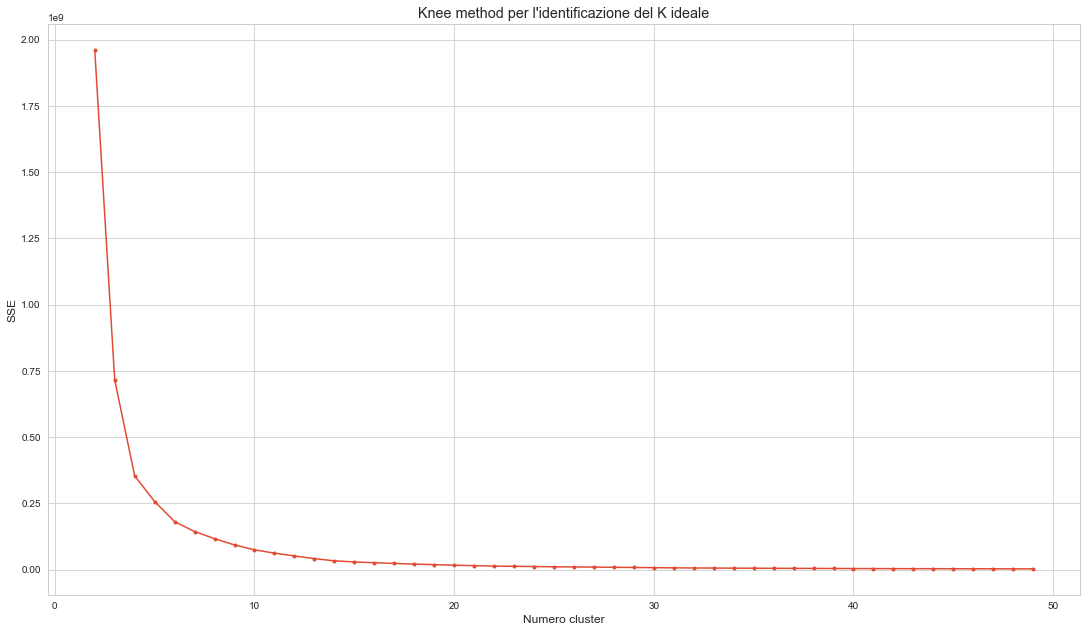
\includegraphics[scale=0.25]{Immagini/SSE.png}
    \caption{SSE con K da 2 a 50}
    \label{fig:SSE}
\end{figure}
\noindent Di seguito il grafico delle \textit{Parallel Coordinates} dei quattro cluster individuati e la tabella che quantifica la popolazione di ciascun cluster. Tutti i cluster sono accomunati da un simile valore medio per \textit{MonthlyIncome} e – a eccezione del Cluster 2 – assenza di \textit{OverTime}. Sempre il Cluster 2 spicca per il \textit{JobLevel} più alto della media. Valori più alti della media si rilevano anche nel Cluster 4 per la \textit{DistanceFromHome}, invece molto bassa per i lavoratori del Cluster 1. 
\begin{figure}[H]
\resizebox{.99\textwidth}{!}{
\centering
\hfill
\begin{minipage}{0.6\textwidth}
  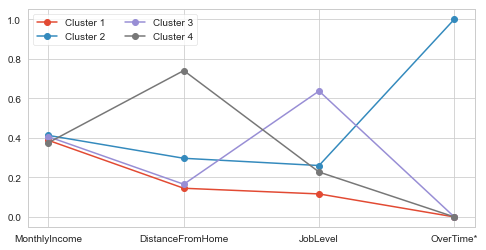
\includegraphics[scale = 0.5]{Immagini/parallelKmeans.png}
    \label{parallelCoord}
    \caption{\textit{Parallel Coordinates} dei \\ cluster}
\end{minipage}
\quad
\begin{minipage}{0.4\textwidth}
\centering
 \begin{tabular}{|c|P{3cm}|}
        \hline    
        \textbf{Cluster} & \textbf{Numero dipendenti nel cluster} \\
        \hline
        0 & 417 \\
        \hline
        1 & 301\\
        \hline
        2 & 137 \\
        \hline
        3 & 174 \\
        \hline
    \end{tabular}
  \captionof{table}{Distribuzione dei dipendenti nei cluster}
\end{minipage}\hspace*{\fill}}
\end{figure}
\noindent\\Si è poi passati a osservare la distribuzione dei vari parametri, a cominciare da \textit{Attrition}. Essa appare pressoché identica fra i Cluster 1 e 4, con una lieve diminuzione nel Cluster 3 e un significativo aumento nel Cluster 2 dovuto, probabilmente, alla presenza di \textit{OverTime} che abbiamo rilevato. I Cluster 2 e 4 contengono inoltre una relativa alta concentrazione di dipendenti con bassa \textit{WorkLifeBalance}.
\\\\
Una possibile spiegazione della bassa concentrazione di \textit{Attrition} nel Cluster 3 – già notato per l’alto \textit{JobLevel} - è data dalla distribuzione di \textit{YearsInCurrentRole}: oltre tre quinti dei dipendenti sono infatti in azienda da più di sei anni. Di contro, i dipendenti del Cluster 1, oltre ad avere un \textit{JobLevel} più basso, sono anche in azienda da meno tempo.
\\\\
I valori di \textit{WorkLifeBalance} e \textit{DistanceFromHome} del Cluster 4 non sembrano essere motivo di \textit{Attrition}, a discapito di quanto si potrebbe pensare intuitivamente (e quanto potrebbe emergere dalla matrice di correlazione). Essi sono forse mitigati dalla concentrazione sopra la media di dipendenti con alto livello di \textit{CompanyInvolvement}.
\\\\
Attributi non direttamente legati alla vita aziendale dell’impiegato, come \textit{MaritalStatus} o \textit{Gender}, risultano invece equamente distribuiti e non degni di nota.
\\\\
Complessivamente, il metodo \textit{K-Means} è riuscito ad analizzare il dataset in modo significativo, mettendo in evidenza alcuni attributi che possono influenzare (in positivo o in negativo) l’\textit{Attrition} dei vari dipendenti.
\begin{figure}[H]
	\centering
	\subfloat 
	{
		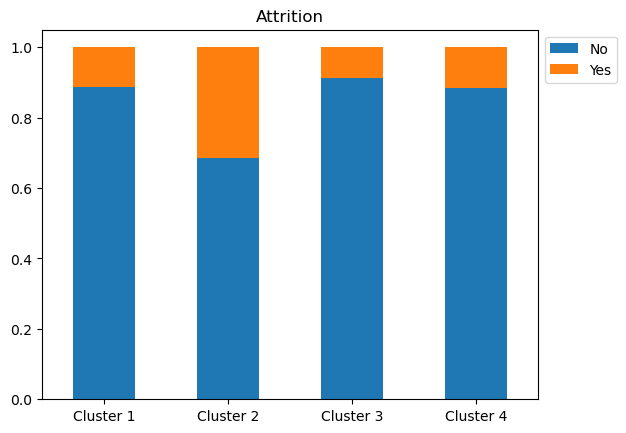
\includegraphics[width=.45\textwidth]{Immagini/KMeansAttr.png}
		\label{kmeansAttrition}
	}
	\quad
	\subfloat
	{
		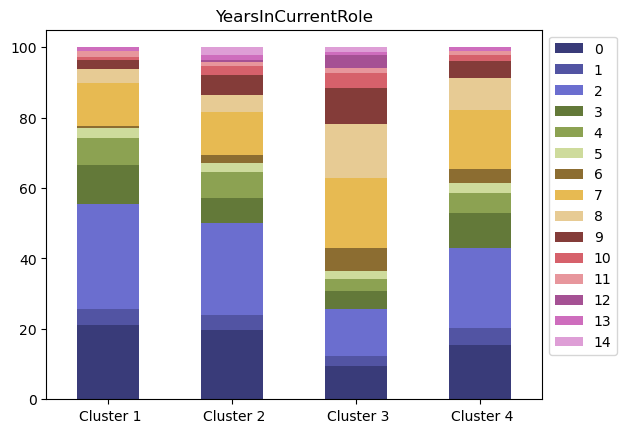
\includegraphics[width=.45\textwidth]{Immagini/KMeansYears.png}
		\label{kmeansYears}
    }
	\label{Cluster}
\end{figure}
\begin{figure}[htp]
\centering
		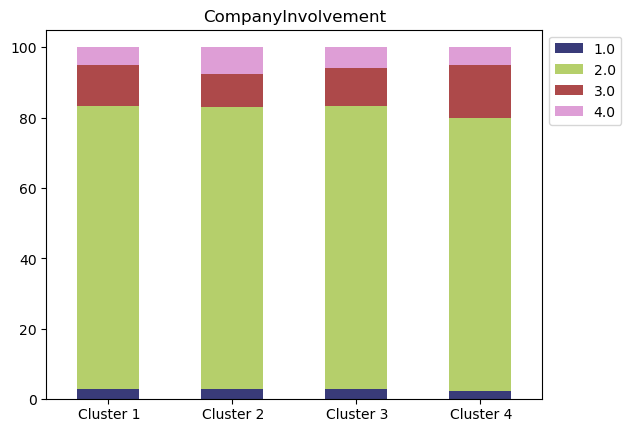
\includegraphics[width=.30\textwidth]{Immagini/KMeansCompanyInv.png}
		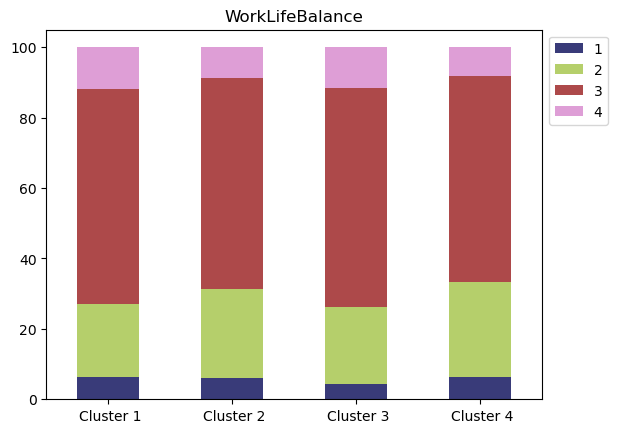
\includegraphics[width=.30\textwidth]{Immagini/KMeansWorkLife.png}
		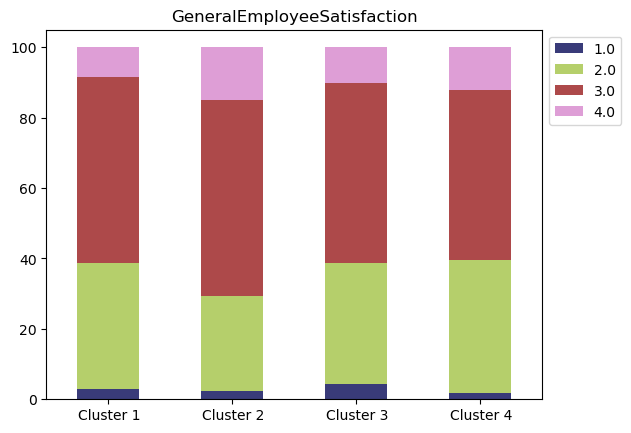
\includegraphics[width=.30\textwidth]{Immagini/KMeansGeneralEmp.png}
		\caption{Distribuzione degli attributi \textit{Attrition}, \textit{YearsInCurrentRole}, \textit{CompanyInvolvement}, \textit{WorkLifeBalance}.\textit{GeneralEmployeeSatisfaction} all'interno dei quattro cluster ottenuti}
\end{figure}
\subsection{\textit{DBSCAN}}
Il metodo di clustering \textit{DBSCAN} si è dimostrato inefficace per il nostro dataset, fortemente sbilanciato con un’alta concentrazione di valori con \textit{Attrition} negativa. L’assunto iniziale – che l'\textit{Attrition} sia determinata da un insieme di più attributi correlati l’un l’altro – sottintende poi un insieme di dati a più dimensioni. Le varie relazioni che intercorrono fra i vari parametri, di cui si è accennato sopra analizzando i risultati del \textit{K-Means}, non possono essere correttamente visualizzate dal \textit{DBSCAN}, che opera in due dimensioni.
\begin{figure}
    \centering
  %  \vspace{-10mm}
    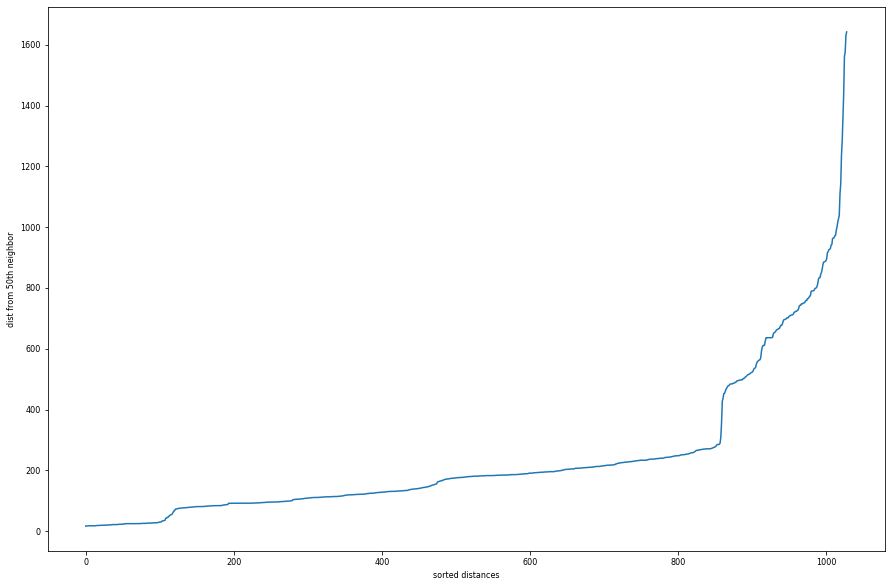
\includegraphics[scale = 0.25]{Immagini/dbscanKnee.png}
    \caption{Grafico \textit{Knee-method}}
    \label{fig:KneeDBSCAN}
    \captionsetup{belowskip=0pt}
\end{figure}                                                                                                                                                                                                                                                                    
\noindent Dopo aver determinato 0.25 come valore ottimale di \textit{EPS} (cioè il raggio dell'intorno di ciascun punto) ricorrendo al \textit{Knee Method} (Fig.\ref{fig:KneeDBSCAN}), si è verificato che l’algoritmo genera il modello con il migliore valore di \text{Silhouette} (0.26) fissando \textit{minPts} (ovvero il numero minimo di punti che un punto deve avere nel suo intorno per essere definito \textit{core}) pari a 4.
\begin{figure}[H]
\resizebox{.99\textwidth}{!}{
\centering
\hfill
\begin{minipage}{0.6\textwidth}
  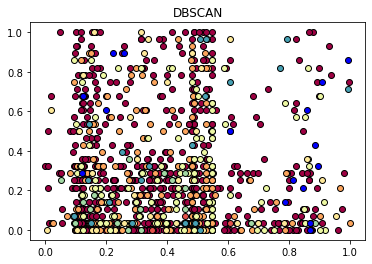
\includegraphics[scale = 0.65]{Immagini/DBSCAN.png}
    
    \caption{\textit{DBSCAN}
    \label{dbScan}}
\end{minipage}
\quad
\begin{minipage}{0.4\textwidth}
\vspace{1em}
\centering
 \begin{tabular}{|c|P{3cm}|}
        \hline    
        \textbf{Cluster} & \textbf{Numero dipendenti} \\
        \hline
        Cluster 1 & 663 \\
        \hline
        Cluster 2 & 7\\
        \hline
        Cluster 3 & 143 \\
        \hline
        Cluster 4 & 44 \\
        \hline
        Cluster 5 & 116\\
        \hline
        Cluster 6 & 19\\
        \hline
        Cluster 7 & 21\\
        \hline
        Rumore & 16 \\
        \hline
        \end{tabular}
  \captionof{table}{Distribuzione dei dipendenti nei cluster}
\end{minipage}\hspace*{\fill}}
\end{figure}
\noindent
Nello spazio sono tuttavia visualizzati dei punti senza alcuna apparente relazione fra loro (Fig. \ref{dbScan}), divisi in otto diversi cluster, di cui uno riservato al rumore. Tali cluster sono molto più sbilanciati di quelli analizzati con il \textit{K-Means}: abbiamo infatti un cluster eccessivamente grande, due medi e gli altri molto piccoli. Analoghi risultati sono stati ottenuti con altri valori di \textit{minPts}.
\\\\
Il basso valore della \textit{Silhouette}, i limiti intrinseci al metodo e lo sbilanciamento dei risultati forniti dal modello fanno propendere contro l’utilizzo del \textit{DBSCAN}.

\subsection{Clustering gerarchico}
Il terzo criterio di clustering sperimentato è quello gerarchico, che a sua volta ammette più possibili applicazioni: sono stati testati alberi gerarchici generati con l’algoritmo \textit{Single Link} (o \textit{MIN}), \textit{Complete} (o \textit{MAX}) e \textit{Average}. In tutti i casi è stato necessario impostare un diverso \textit{threshold} per ottenere un certo numero di cluster. Nel nostro caso, dovendo confrontare i risultati del metodo gerarchico con quelli ottenuti mediante \textit{K-Means}, abbiamo cercato di ottenere sempre quattro cluster.

\begin{table}[H]
\centering
\begin{tabular}{|l|c|c|S|}
\hline
\multicolumn{1}{|c|}{\textbf{Metodo}} & \multicolumn{1}{c|}{\begin{tabular}[c]{@{}c@{}}\textbf{Grandezza} \\ \textbf{cluster}\end{tabular}} & \multicolumn{1}{c|}{\textbf{Threshold}} & \multicolumn{1}{c|}{\textbf{Silhouette}} \\ \hline
Complete   & 69, 232, 180, 548   & 1.4  &   0.33777407417668387          \\ \hline
Average           & 726, 293, 8, 2   & 0.85    &    0.3784611202348606    \\ \hline
Single           & 728, 298, 2, 1   & 0.28 &  0.44019713225483575   \\  \hline
\end{tabular}
\caption{Differenti parametri impostati per il clustering gerarchico}
\end{table}

\begin{figure}[H]
\centering
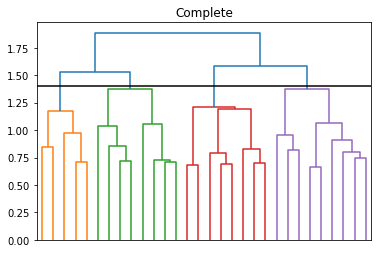
\includegraphics[width=.3\textwidth]{Immagini/GeraComplete.png}\hfill
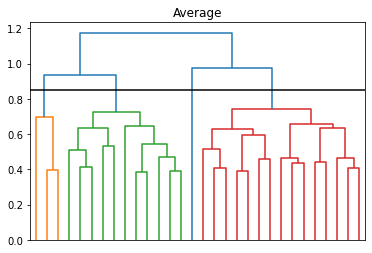
\includegraphics[width=.3\textwidth]{Immagini/GeraAvg.png}\hfill
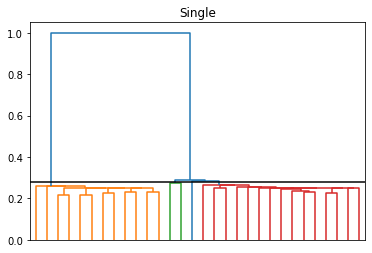
\includegraphics[width=.3\textwidth]{Immagini/GeraSingle.png}
\caption{Cluster gerarchici ottenuti con i metodi \textit{Complete}, \textit{Average} e \textit{Single link}}
\label{fig:clusterGerarchico}

\end{figure}
\noindent I risultati sono stati soddisfacenti solo con il metodo \textit{Complete}. Negli altri casi i cluster risultano sbilanciati, con due cluster contenenti un numero molto basso di oggetti, un cluster eccessivamente grande e un cluster medio. A questo fenomeno vi sono due possibili spiegazioni. \\\\Da una parte, poiché simili risultati sono stati ottenuti anche cercando differenti quantità di cluster, il problema potrebbe essere legato allo stesso dataset: l’alta quantità di rumore avrebbe portato gli algoritmi a costruire delle enormi “catene” incapaci di rilevare validi raggruppamenti per i diversi oggetti. Un'altra possibile spiegazione è che effettivamente sia preferibile avere due grandi cluster, situazione a cui \textit{de facto} hanno portato i due metodi gerarchici. Il clustering generato dal metodo \textit{Single Link} mostra poi un alto valore di \textit{Silhouette}, coerentemente con quanto notato testando il \textit{K-Means} impostando \textit{K} pari a 2. Operare con solo due cluster, però, impedirebbe analisi più dettagliate dei diversi fattori che influenzano \textit{Attrition}.
\\\\I risultati ottenuti dal metodo \textit{Complete}, comunque, non confermano quelli del \textit{K-Means}. La distribuzione degli oggetti è, nel complesso, diversa: nel \textit{K-Means}, ad esempio, avevamo un solo cluster con ampia concentrazione di impiegati con \textit{OverTime}.




\subsection{Conclusioni sul clustering} Dalla nostra analisi l’algoritmo di clustering più efficace per l’analisi del dataset si è dimostrato il \textit{K-Means}. Lo sbilanciamento del dataset e la forte presenza di rumore hanno reso impossibile applicare con risultati significativi i metodi \textit{DBSCAN}, \textit{Gerachico Single-Link} e \textit{Gerarchico Average}. Risultati migliori sono stati ottenuti dal \textit{Gerarchico Complete}, la cui \text{Silhouette} è tuttavia più bassa di quella del \textit{K-Means}.
\vspace{5mm}
\begin{table}[H]
\centering

\begin{tabular}{|l|c|c|}
\hline
\textbf{Algoritmo}                                              & \textbf{Silhouette} \\ \hline
\textit{K-Means}                                                         & 0.397               \\ \hline
\textit{DBSCAN}                                                          & 0.26                \\ \hline
\begin{tabular}[c]{@{}c@{}}Gerarchico\\ (\textit{Complete})\end{tabular} & 0.338               \\ \hline
\end{tabular}
\caption{Tabella riassuntiva sugli algoritmi di clustering applicati e migliori valori della \textit{Silhouette}}
\end{table}